\documentclass[12pt]{article}   	

% Document Formatting Packages
\usepackage{geometry}            		
\geometry{letterpaper}  
\usepackage[usenames,dvipsnames,svgnames,table]{xcolor}


% Document Navigation Packages
\usepackage[parfill]{parskip}          
\usepackage{enumitem}         

% Math Typesetting Tools
\usepackage{amssymb}
\usepackage{amsmath,mathtools}
\usepackage{framed}

% Hyperref
\usepackage[colorlinks=true,linkcolor=blue,citecolor=red]{hyperref}

% Chemistry Typesetting Tools
\usepackage[version=4]{mhchem}

% Inserting Figures
\usepackage{graphicx}
\usepackage[section]{placeins}
\graphicspath{ {images/} }	
\usepackage[caption=false]{subfig}		

% Miscellaneous Symbol Packages
\usepackage{textcomp}  		
\usepackage{siunitx}
\usepackage{gensymb}

% Set Document Dimensions
\oddsidemargin = 0in
\topmargin = 0in
\headheight=0pt
\headsep = 0pt
\textheight = 9in
\textwidth = 6.5in
\marginparsep = 0in
\marginparwidth = 0in
\footskip = 18pt
\parindent=15pt
\parskip=0pt

\hypersetup{
	%bookmarks=true,         % show bookmarks bar?
	pdfauthor={},     		 % author
	colorlinks=true,       	 % false: boxed links; true: colored links
	linkcolor=blue,          % color of internal links
	citecolor=red,           % color of links to bibliography
}

% Title
\title{Weekly Update - Week of 10 June 2018}
\author{Joseph Lucero}
\date{\today}

\begin{document}
\maketitle

\section{Past Week}

This \textbf{past week} I was focused on \textbf{two} primary tasks:
\begin{enumerate}
	\item \textbf{Track down why the 2mm results gave funny behaviours while 1mm results did not}
	\begin{itemize}
		\item After some investigation I have finally figured out why the dose distributions for the 2mm case did not give the correct results
		\item I finally realized that in order for volume corrections to take into account the fact that an applicator is present and thus correct for it you must \underline{set the applicator geometry} \underline{as a source geometry} in addition to the seed geometry \emph{during volume corrections}
		\item However, strictly speaking, only the \ce{^{192}Ir}, is emitting radiation. Thus, \emph{during the simulation of radiation transport}, the \underline{source must be set only to the \ce{^{192}Ir} (seed) geometry}
		\item Examples that ship with egs\_brachy do not do this for some reason
		\begin{itemize}
			\item Not sure why this problem wasn't encountered in the example HDR case
			\item Might be because the doses that were measured were fairly far away from the applicator?
		\end{itemize}
		\item Having done this I now get good (differences of at most 8\%) agreement with Lymperopoulou results. 
		\begin{itemize}
			\item I think once I have the error bars in place the small difference from expected can be explained 
		\end{itemize}
	\end{itemize}
	\item \textbf{Read Peppa et al. (2016) paper and explore data set available}
	\begin{itemize}
		\item Read the Peppa paper once through
		\item Need to read again for clarification on models and test cases
		\item Downloaded the data sets from the Radiation Dosimetry Lab (RDL) website
		\item Used a Python parser (Python module: dicom) to see what was in the dicom files
		\item Looked over Stephen's scripts a bit to figure out how he turned these dicom files into egsphants
		\item Still need more time to process Stephen's code
	\end{itemize}
\end{enumerate}

\section{Next Week}

This \textbf{next week} I will be focused on \textbf{three} primary things:
\begin{enumerate}
	\item \textbf{Doing Data Production Runs}
	\begin{itemize}
		\item With the problem of volume corrections having been solved and everything else seeming okay, I am ready to do runs for all different sizes of applicators and for the three different sources
		\item Will probably have most of them run on Graham
		\item Might also expand to Cedar cluster depending on if the simulations get too many
		\item If I have time, I may replicate Joanna's configuration of dwell positions as well
	\end{itemize}
	\item \textbf{Add errors and error propagation to my analysis}
	\begin{itemize}
		\item Need to add error bars to all my plots
		\item Having a little bit of trouble figuring out the correct way to do it
		\item Looking at code for how 3D Dose Tools does error propagation
		\item Will converse with Martin this week to try and sort the algorithm out
	\end{itemize}
	\item \textbf{Work at reproducing Case 3 of Peppa paper}
	\begin{itemize}
		\item As a start/benchmark, will first look at recreating Case 3
		\item Try and get an understanding of the results 
		\item Work out pipeline in Python that will get me from CT dicom files to egsphant
	\end{itemize}
\end{enumerate}

\section{Figures}

\begin{figure}
	\centering
	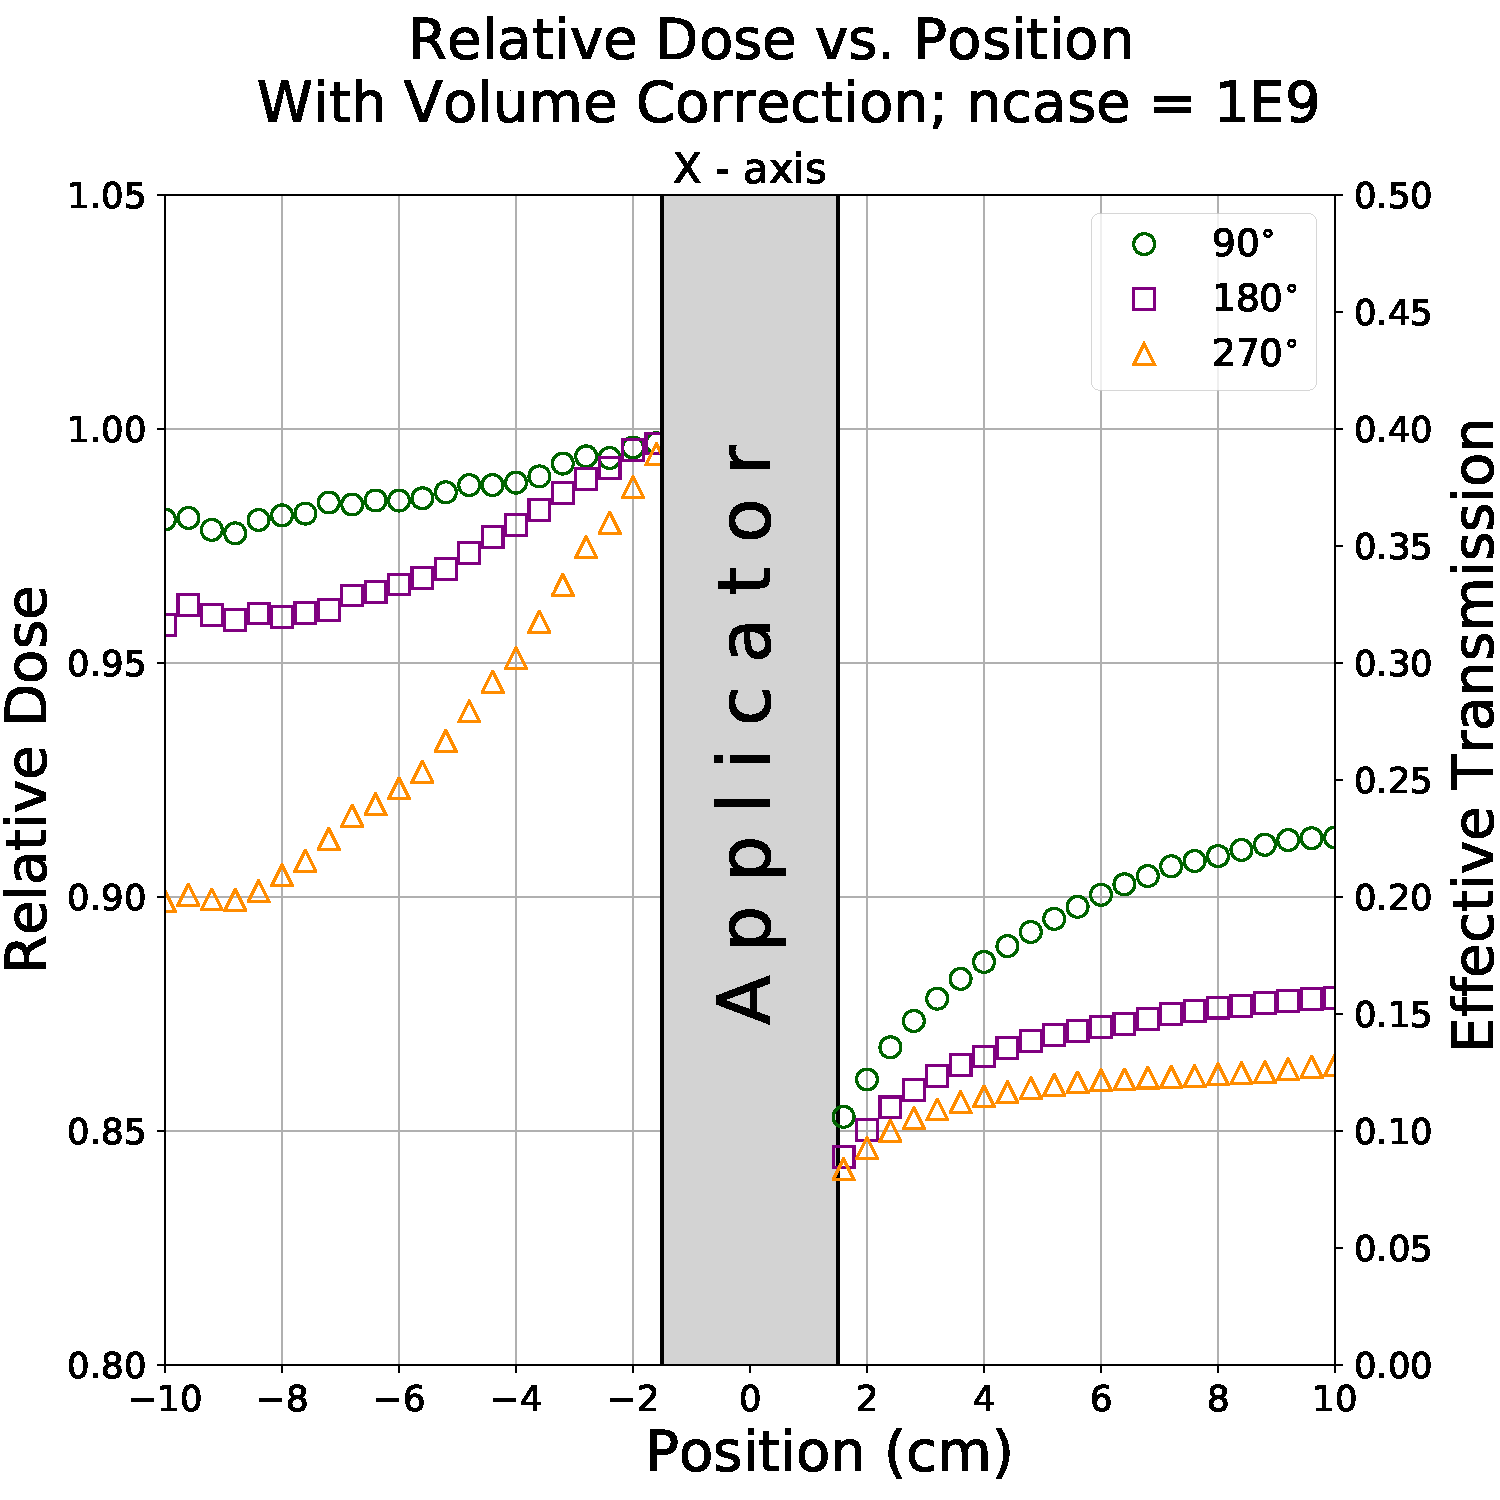
\includegraphics[scale=0.3]{relative_dosage_comparison}
	\caption{\textbf{Relative Dose Comparison}. MC calculated results of dose for a shielded applicator to dose for the unshielded applicator at the same point as a function of distance away, x, for y=0 cm in the unshielded (relative dose, left) and the shielded (transmission factor, right) sides of the central axial plane (xy at z=0 cm) for the $ 90\degree $ (green circles), the $ 180\degree $ (purple squares), and the $ 270\degree $ (orange triangles) tungsten alloy shields.}
\end{figure}

\FloatBarrier

\begin{table}[]
	\centering
	\caption{Shielded side comparison of attenuation factors}
	\label{my-label}
	\begin{tabular}{|c|c|c|c|c|}
		\hline
		Shield Type & X-Coord & Relative Dose   & Expected & Difference (\%) \\
		\hline
		90          & 10      & 0.2225405158618 & 0.23     & 3.243           \\
		\hline
		180         & 10      & 0.156912113441  & 0.17     & 7.69            \\
		\hline
		270         & 10      & 0.128142220894  & 0.13     & 1.43            \\
		\hline
	\end{tabular}
\end{table}   	

\end{document}